\documentclass{llncs}
\pagestyle{plain}
\usepackage[english]{babel}
\usepackage[utf8x]{inputenc}
\usepackage{amsmath}
\usepackage{graphicx}
\usepackage{url}
\usepackage[colorinlistoftodos]{todonotes}

\makeatletter
\newcommand*{\bdiv}{%
  \nonscript\mskip-\medmuskip\mkern5mu%
  \mathbin{\operator@font div}\penalty900\mkern5mu%
  \nonscript\mskip-\medmuskip
}
\makeatother

\title{Capturing the Ineffable:\\Collecting, Analysing and Automating Web Document Quality Assessments}
% * <j.j.noordegraaf@uva.nl> 2016-07-17T10:22:37.847Z:
%
% > Ineffable
%
% I think this term is not the best; see my suggestions below.
%
% ^.
\author{Davide Ceolin\inst{1} and Lora Aroyo\inst{1} and Julia Noordegraaf\inst{2}}
\institute{\email{\{d.ceolin,lora.aroyo\}@vu.nl}\\VU University Amsterdam\\ de Boelelaan 1081a\\ 1081HV\\ Amsterdam, The Netherlands \and \email{j.j.noordegraaf@uva.nl} \\ University of Amsterdam}

\begin{document}
\maketitle
\begin{abstract}
Automatic estimation of the quality of Web documents is a challenging task, especially because the definition of quality heavily depends on the individuals who define it, on the context where it applies, and on the nature of the tasks at hand. 
In this paper, we investigate the characteristics of Web documents that hint at their quality as follows: (1) we define features of Web documents that may be indicators of quality;  (2) we design a procedure for automatically extracting those features; (3) develop a Web application to present these results to niche users to check the relevance of these features as quality indicators and collect quality assessments;  (4) we analyse user's qualitative assessment of Web documents to refine our definition of the features that determine quality, and establish their relevant weight in the overall quality.
Hence, our contributions are threefold: a Web application for nichesourcing quality assessments; a curated dataset of Web document assessments; and a thorough analysis of the quality assessments collected by means of two case studies involving experts (journalists and media scholars).
%Firstly, we propose a method for capturing Web quality assessments based on a nichesourcing Web application that we developed. Secondly, we investigate the characteristics of Web documents that hint at their quality levels. We identify features of Web documents that may indicate quality, we propose a model for automatically estimating such assessments, we analyze users ability to judge quality based on features extracted from these documents and, finally, we decompose overall quality assessments so to identify which quality dimensions (e.g., accuracy, precision) are of higher importance when assessing Web documents.
% * <j.j.noordegraaf@uva.nl> 2016-07-15T07:27:26.765Z:
%
% > We propose a model for automatically estimating such assessments, we analyze users ability to judge quality based on features extracted from these documents and, finally, we decompose overall quality assessments so to identify which quality dimensions (e.g., accuracy, precision) are of higher importance when assessing Web documents
%
% So after the aim, we outline the method with which we will do it: 1. defining features of web docs that may be indicators of quality;  2. design a procedure for automatically extracting those; 3. presenting the results to users to check the relevance of these features as quality indicators; 4.  analyse user's qualitative assessment of web docs so refine our definition of the features that determine quality, and establishing their relevant weight in the overall quality.
%
% ^ <davide.ceolin@gmail.com> 2016-07-17T12:41:26.474Z:
%
% Done
%
% ^ <davide.ceolin@gmail.com> 2016-07-17T12:47:01.586Z.
% * <j.j.noordegraaf@uva.nl> 2016-07-15T07:22:52.077Z:
%
% > Secondly
%
% Perhaps first and second should be presented the other way around; investigating the characteristics of web documents that hint at their quality is a more general aim (is it a 'perspective?') and proposing a method for capturing the assessment of these quality levels another that follows from the first.
%
% ^ <davide.ceolin@gmail.com> 2016-07-17T12:41:20.899Z:
%
% Done
%
% ^ <davide.ceolin@gmail.com> 2016-07-17T12:47:03.063Z.
%We tested our approach in two use cases involving experts (journalists and media scholars) that make professional use of Web documents. 
%DONE
These analyses show that: (1) it is possible to automate the process of Web document quality estimation to a level of high accuracy; (2) document features shown in isolation are poorly informative to users; and (3) related to the tasks we propose (i.e., choosing Web documents to use as a source for writing an article on the vaccination debate), the most important quality dimensions are accuracy, trustworthiness, and precision.
\end{abstract}

\section{Introduction}
Automatically estimating the quality of Web documents is a compelling, yet intricate issue. It is compelling because the huge amount of Web documents we can access makes their manual evaluation a costly operation. So, to guarantee we access the best documents available on the Web on a given matter, an automated assessment is needed. 
However, quality is a rather inflated term, that assumes different meanings in different contexts and with different subjects. Quality assessments vary depending on their context (what is the document assessed used for), author (who is judging the document), time (e.g., users may change their assessments about documents as soon they acquire new knowledge), etc. Quality assessments are hard to capture, hence we call them ``ineffable''.

This paper investigates how it is possible to capture such ineffable judgments and how they are characterized. In particular, our current focus is on the quality assessment of Web documents to be used for professional use (i.e., by journalists and media scholars). 
The contribution of this paper is threefold. Firstly, we introduce a nichesourcing application for collecting Web document quality assessments (WebQ\footnote{The tool is running at \url{http://webq3.herokuapp.com}, the code is available at~\url{https://github.com/davideceolin/webq}.}). Secondly, we present a curated dataset of Web documents (on the topic of vaccinations) enriched with a set of features we extracted, and a set of quality assessments we nichesourced\footnote{The dataset of enriched documents is available at~\url{https://github.com/davideceolin/WebQ-Analyses}.}. Thirdly, we describe a thorough set of analyses we performed on these quality assessments, from which we derive that: (1) given an explicit task at hand, subjects with similar background will provide coherent assessments (i.e., assessments agree with document similarity, measured in terms of shared entities, sentiment, emotions, trustworthiness);
% * <j.j.noordegraaf@uva.nl> 2016-07-15T07:52:33.174Z:
%
% > threefold
%
% see below; here it seems to make more sense to discuss it in this order; check what works best and match with abstract
%
% ^ <davide.ceolin@gmail.com> 2016-07-16T15:05:43.028Z:
%
% Done
%
% ^ <davide.ceolin@gmail.com> 2016-07-17T12:47:08.057Z.
%DONE
(2) users find it difficult to judge document quality based on quantitative features (entities, sentiment, emotions, trustworthiness) extracted from them; however (3) such features are useful to automate the process of quality assessment.%; (4) the relevance of different quality dimensions to the users strictly depends on the task at hand.
% * <j.j.noordegraaf@uva.nl> 2016-07-15T07:55:44.235Z:
%
% > (4) the relevance of different quality dimensions to the users strictly depends on the task at hand.
%
% One and four are the same; in one, I do not quite understand what the difference is between a task and the subjective evaluation?
%
% ^ <davide.ceolin@gmail.com> 2016-07-16T15:05:54.971Z:
%
% done
%
% ^ <davide.ceolin@gmail.com> 2016-07-17T12:47:09.855Z.
% * <j.j.noordegraaf@uva.nl> 2016-07-15T07:55:02.385Z:
%
% > their learning
%
% what is 'their' referring to? to automate the extraction? not clear what is meant
%
% ^ <davide.ceolin@gmail.com> 2016-07-16T15:06:02.695Z:
%
% done
%
% ^ <davide.ceolin@gmail.com> 2016-07-17T12:47:11.287Z.
%DONE

The rest of the paper is structured as follows. Section~\ref{sec:related} introduces related work. Section~\ref{sec:webq} describes the nichesourcing Web application we developed for collecting quality assessments, WebQ.
Section~\ref{sec:results} describes the two case studies we performed, along with the results collected. These results are discussed in Section~\ref{sec:discussion}. Section~\ref{sec:conclusion} concludes the paper.


\section{Related Work}
\label{sec:related}

The problem of assessing the quality of Web documents and, in general, (Web) data and information, is compelling, and has been tackled in many contexts. 

The ISO 25010 Model~\cite{iso} is a standard model for data quality. From this model, we select those data quality dimensions that apply also to Web documents (e.g., precision, accuracy) and ask the users of WebQ to rate Web documents on them. This set of quality dimensions has been extended to include other measures tailored to Web documents, like neutrality and readability.

The problem of identifying the documents of higher quality for a given purpose is common in information retrieval. Bharat et al~\cite{bharat2016method} copyrighted a method for clustering online news content based on freshness and quality of content. Clearly, their approach differs from ours as they focus on news, and they aim at clustering documents. However, one of the key features for determining the quality of documents is the (estimated) authoritativeness of the source, both in their and in our approach. Kang and Kim~\cite{Kang:2003:QTC:860435.860449} find links between specific quality requirements and user queries. We do not make use of queries: we preselect documents (to guarantee that documents get an even number of assessments) and we predefine the task the users are asked to perform (to allow controlling the definition of quality adopted by users). We still analyze user assessments to derive their specific definition of quality, and might consider analyzing user queries in the future, when we will expand the dataset and tasks at hand.
% * <j.j.noordegraaf@uva.nl> 2016-07-15T08:00:03.504Z:
%
% > We do not make use of queries since we preselect documents and also predefine the task the users are asked to perform. 
%
% Can we motivate this decision?
%
% ^ <davide.ceolin@gmail.com> 2016-07-17T12:41:46.719Z:
%
% Done
%
% ^ <davide.ceolin@gmail.com> 2016-07-17T12:47:16.025Z.
Following up on the use of specific metadata as markers for quality, Amento et al.~\cite{Amento:2000:LMQ:345508.345603} use link-based metrics to make quality predictions, showing that these perform as good as content-based ones. In our case, we focus on features we can automatically extract from the documents using AlchemyAPI and WOT. We will consider other features (including link-based ones) in the future. %mainly on metadata- and context-based features, and will consider link-based ones in the future.
% * <j.j.noordegraaf@uva.nl> 2016-07-15T08:01:21.967Z:
%
% > we focus mainly on metadata- and context-based features, and will consider link-based ones in the future.
%
% It seems we just did not get to this yet; is there a better motivation for not (yet) considering link-based metrics?
%
% ^ <davide.ceolin@gmail.com> 2016-07-17T12:42:06.795Z:
%
% Done
%
% ^ <davide.ceolin@gmail.com> 2016-07-17T12:47:18.310Z.
%DONE

Regarding the use of niche- or crowdsourcing for collecting information and, in particular, quality assessments, Lee et al.~\cite{Lee:2002:AMI:637474.637478} provide a framework tailored to organizations. Zhu et al.~\cite{zhu} propose a method for collaboratively assessing the quality of Web documents that shows some similarity with ours (e.g., we both collect collaborative quality assessments), but the assessments we aim at collecting are based on specific tasks, while they rely on contributions via browsers plugins. Currently, we focus on niches for collecting quality assessments because the definition of 'quality' is different for different types of users; so, for us, it is necessary to have a controlled user study. In the future, we will make use of crowdsourcing as well, embracing methods for extracting ground truth like the CrowdTruth framework~\cite{Inel2014}.
% * <j.j.noordegraaf@uva.nl> 2016-07-15T08:04:34.738Z:
%
% >  we focus on niches for collecting quality assessments
%
% this is motivated by the fact that the definition of 'quality' is different for different types of users; so for us it was necessary to have a controlled user study.
%
% ^ <davide.ceolin@gmail.com> 2016-07-17T12:42:15.672Z:
%
% Done
%
% ^ <davide.ceolin@gmail.com> 2016-07-17T12:47:20.457Z.
%DONE


While this paper proposes a framework that aims at generically identifying markers for quality of Web documents, we evaluate such framework with an emphasis on Digital Humanities applications. Digital Humanities scholars are professionals that are used to critically evaluate the sources they deal with, hence we target this specific class of users to investigate how to extend source criticism practices to cover Web documents as well.
Source criticism is the process of evaluating traditional information sources that is common in the (Digital) Humanities. De Jong and Schellers~\cite{dejong} provide an overview of source criticism methods, evaluated in terms of predictive and congruent validity. We will advance such evaluations to identify which Web document features determine their quality.
This paper extends the work we presented at the Web Science conference, where we began the exploration of how it is possible to assess the quality of Web documents, especially for the Digital Humanities~\cite{Ceolin:2016:TWD:2908131.2908198}.

Lastly, one aspect that we partially consider when estimating the quality of Web document is their provenance. Provenance analysis is used to assess the quality of humanities sources, as Howell and Prevenier mention~\cite{provenance}. In Computer Science,
the use of provenance information to assess the quality of Web data has been explored by Hartig and Zhao~\cite{hartig}, who focus mostly on temporal qualities. More extensively, Zaveri et al.~\cite{LDQ} provide a review on quality assessment for Linked Data. We also investigated the assessment of crowdsourced annotations using provenance analysis~\cite{jdiq2015,ifiptm2015}. 

\section{Nichesourcing Web Document Quality Assessments}
\label{sec:webq}
To collect and analyse judgments about Web documents, we developed the tool WebQ, that aims at understanding three main aspects of Web document quality:
\begin{itemize}
\item  whether (professional) users are able to estimate the quality of Web documents based on limited sets of features of these documents (e.g., the sentiment of these documents, or the list of entities extracted from them);
\item  whether assessments are coherent enough over multiple documents and among diverse assessors (i.e., different assessors assess similar documents in a similar manner; similarity is measured in terms of shared entities, sentiment, emotions, trustworthiness), to allow their automated learning;
% * <j.j.noordegraaf@uva.nl> 2016-07-15T08:12:25.908Z:
%
% > their automated learning
%
% Again, unclear; do you mean whether the judgments are coherent enough to automate them?
%
% ^ <davide.ceolin@gmail.com> 2016-07-17T12:42:30.935Z:
%
% Done
%
% ^ <davide.ceolin@gmail.com> 2016-07-17T12:47:24.905Z.
%DONE
\item  how the overall quality assessments can be explained in terms of specific quality dimensions (precision, accuracy, etc.) when focusing on specific tasks.
% * <j.j.noordegraaf@uva.nl> 2016-07-15T08:11:45.964Z:
%
% > how the overall quality assessments of Web documents can be explained in terms of specific quality dimensions (i.e., understanding what is the weight of precision, accuracy, etc. when users provide overarching quality assessments about Web documents), when focusing on specific tasks
%
% perhaps this sentence can be rephrased to make it a bit more clear and concise
%
% ^ <davide.ceolin@gmail.com> 2016-07-17T12:42:36.173Z:
%
% Done
%
% ^ <davide.ceolin@gmail.com> 2016-07-17T13:12:08.877Z.
%DONE
\end{itemize}

\subsection{Document Features and Document Quality Dimensions}
We characterize documents by means of features we automatically extract about them. In Section~\ref{sec:results} we analyze the existence of correlations between these automatically extracted features and the nichesourced features of quality.
\subsubsection{Document Features} These are a series of attributes we automatically extract by means of Web APIs. These features aim at identifying commonalities among documents, opening up for the possibility of predicting their qualities (provided that features and qualities correlate). These features are:
% * <j.j.noordegraaf@uva.nl> 2016-07-15T08:14:57.244Z:
%
% > These features are:
%
% the titles of the features should also be indented, to distinguish from the 'document features' header above
%
% ^ <davide.ceolin@gmail.com> 2016-07-17T13:12:11.350Z.
% DONE (it is not possible to indent, I wrote them in italic)
\begin{description}
\item[{\it Entities, Sentiment, Emotions}] We use AlchemyAPI\footnote{\url{http://www.alchemyapi.com}} to extract all the features mentioned in the documents, along with an assessment of their relevance to the document. Also, AlchemyAPI provides us with a quantification of the sentiment expressed by the document (positive or negative, and its strength), and its emotions (joy, fear, sadness, disgust and anger, and their strength).
\item[{\it Trustworthiness}] In this case, we use the Web Of Trust API\footnote{\url{http://www.mywot.com}} to obtain crowdsourced trustworthiness assessments about the source publishing the article.
% * <j.j.noordegraaf@uva.nl> 2016-07-15T08:16:11.143Z:
%
% > This is an anomalous feature, because trustworthiness belongs also to the document qualities
%
% I'm not sure I understand what is meant here
%
% I'm not sure I understand what is meant here
%
% ^ <j.j.noordegraaf@uva.nl> 2016-07-15T08:17:05.054Z:
%
% If it is anomalous , why then discuss it here and not below?
%
% ^ <davide.ceolin@gmail.com> 2016-07-17T13:12:27.984Z.
%DONE
\end{description}
\subsubsection{Document Quality Dimensions} These are a series of abstractions of the documents qualifying the information therein contained. We ask the users to assess the documents based on each quality dimension reported as follows:
\begin{description}
\item[Overall Quality] represents the overall reliability of the document.
% * <j.j.noordegraaf@uva.nl> 2016-07-15T08:17:20.000Z:
%
% > overall reliability
%
% defined as...?
%
% ^ <davide.ceolin@gmail.com> 2016-07-17T13:12:32.290Z.
%DONE
\item[Accuracy] quantifies the level of truthfulness of the document information.
\item[Precision] quantifies whether the document information is precise.
\item[Completeness] determines whether the document information is complete.
\item[Neutrality] determines whether a particular stance (e.g., pro or con a given topic) is represented in the document.
\item[Readability] quantifies whether the document reads well.
\item[Trustworthiness] quantifies the perceived level of trustworthiness of the information in the document. Note that the Web Of Trust score refers to the source, while this quality refers to the specific document evaluated.
% * <j.j.noordegraaf@uva.nl> 2016-07-15T08:18:48.836Z:
%
% > uantifies the level of truthfulness of the document information.
% > \item[Precision] quantifies whether the document information is precise.
% > \item[Completeness] determines whether the information contained in the document (or facts) are complete.
% > \item[Neutrality] determines whether a particular stance (e.g., pro or con a given topic) is represented in the document.
% > \item[Readability] quantifies whether the document reads well.
% > \item[Trustworthiness] quantifies the perceived level of trustworthiness of the information in the document. Note that the Web Of Trust score refers to the source, while this quality refers to the specific document evaluated.
%
% For each, I feel it would be good to add how they are defined/determined. So what does 'complete' or 'reading well' mean, exactly? So what does the software take into account to determine the degree to which these features are there?
%
% ^ <davide.ceolin@gmail.com> 2016-07-17T13:12:36.917Z.
%DONE. These are the quality dimensions we ask the users to evaluate, so there is no software extracting them in this case.
\end{description}


\subsection{Structure of WebQ}

Below we describe the structure of WebQ, illustrated in Figure~\ref{fig:overview}.
\paragraph{Architecture}
The application is developed based on the Flask Python library\footnote{\url{http://flask.pocoo.org/}}.
As backend storage for Web document assessments, we use MongoDB\footnote{\url{http://mongodb.com}}.
\paragraph{Annotations}
We use AnnotatorJs\footnote{\url{http://annotatorjs.org}} as a tool allowing users to indicate which specific parts of a document mark particular qualities of the whole document.
AnnotatorJs is a javascript library ran on the client side. This library records the document annotations by sending HTTP messages to a storage server. We adapted to this purpose the Annotation Store\footnote{\url{https://github.com/openannotation/annotator-store}}, which relies on ElasticSearch for storage and retrieval of annotations.
\paragraph{HTTP Proxy}
We developed an HTTP proxy to provide the users with the Web documents to be annotated within WebQ. This proxy allows to present the documents within our application and allows users to annotate them by enabling AnnotatorJs. In this manner, the users see the exact same document they would see on the Web, but they are able to annotate it, remaining in the context of our application.
This proxy is tailored to the documents in our dataset and renders them at their best. In particular, it addresses the following issues:
\begin{description}
\item[replace relative paths with absolute ones] in image, CSS and link addresses, so that the page can refer to the absolute addresses of the accessory files;
\item[correctly detect and utilize charsets] to properly render the documents;
\item [forward the browser headers] because some websites allow being accessed only via (some) browsers, and not being scraped. The proxy accesses them programmatically on behalf of a browser.%, the proxy  forwards the browser headers to the website.
\end{description}
In the future, we will extend our dataset, so we will extend further this proxy.
\paragraph{Randomizer}
WebQ is designed for collecting Web document quality assessments via one or more user studies. In such a scenario, users access the application more or less simultaneously. We assign to each user a random sequence of documents to assess (we set the length of such sequence to six), but we also guarantee that the dataset is uniformly assessed: documents should get approximatively $$ n_{assessments} = |dataset |  \bdiv | {\it users} | $$ assessments, where $| dataset|$ is the cardinality of the document dataset (50), $\bdiv$ is the integer division and $| {users}|$ is the cardinality of the set of users. 
Before running the user studies, we generate $n_{assessments}$ random permutations of documents. We split such sequences in consecutive sequences of six documents. Sequences are uniquely assigned to users as soon as they register.

\begin{figure}
\centering
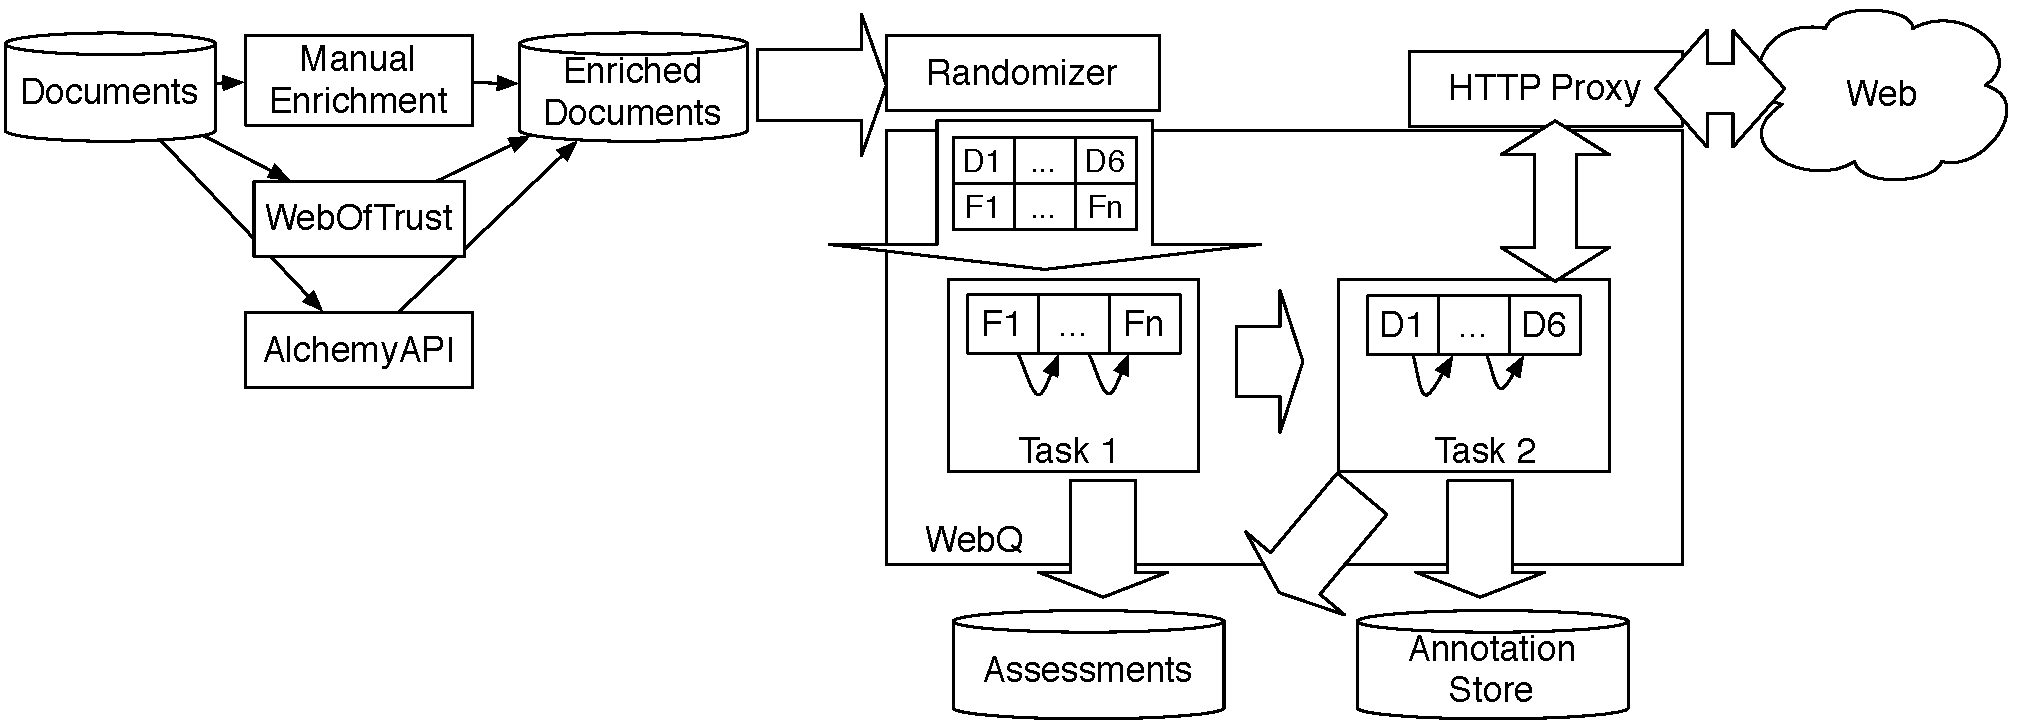
\includegraphics[width=0.95\textwidth]{overview.pdf}
\caption{Overview of the WebQ application. The document set is enriched by using AlchemyApi, Web of Trust, and manually. A random selection of six documents is presented to the users for the first task: identifying the highest quality documents on the basis of the value of one feature. After all the features (sentiment, etc.) have been evaluated, users assess each of the six documents assigned (task 2). Documents are rendered through an HTTP proxy, to allow annotating them within the app.\label{fig:overview}}
\end{figure}

\subsection{Tasks Description}
In WebQ we ask the users to perform two tasks. The first task aims at exploring whether single document features could be used as quality indicators. The second task aims at collecting assessments about the documents presented. The two tasks are described as follows, first in general terms, and then, in section 4, as adapted according to a specific scenario for the two case studies.
% * <j.j.noordegraaf@uva.nl> 2016-07-15T08:36:29.230Z:
%
% > first in general terms, and then, in section 4, as adapted according to a specific scenario for the two case studies
%
% I added this because it feels aspects of the actual cases are missing from this description (such as the description of the task, namely that they are instructed to select docs relevant for writing an article on vaccination). I understand you want to discuss the setup in more general terms first but  that it also has a specific instruction for users in practical applications should perhaps be indicated?
%
% ^ <davide.ceolin@gmail.com> 2016-07-17T13:12:47.037Z.
% * <j.j.noordegraaf@uva.nl> 2016-07-15T08:31:33.162Z:
%
% > whether single document features could be used as quality indicators
%
% I changed this; is this rephrasing correct?
%
% ^ <davide.ceolin@gmail.com> 2016-07-17T13:12:45.818Z.
% DONE

\paragraph{Task 1}
%The application is divided into two tasks. In the first, task we evaluate the informativeness of specific document features in relation to the quality of the documents.
% * <j.j.noordegraaf@uva.nl> 2016-07-15T08:32:40.056Z:
%
% > The application is divided into two tasks. In the first, task we evaluate the informativeness of specific document features in relation to the quality of the documents.
%
% You explain this in the previous paragraph; leave out here?
%
% ^ <j.j.noordegraaf@uva.nl> 2016-07-15T08:33:20.524Z:
%
% Or say something about task 1 only here, if useful
%
% ^ <davide.ceolin@gmail.com> 2016-07-17T13:12:50.117Z.
%DONE
Task 1 is structured as follows:
\begin{enumerate}
\item We assign to each user a set of six documents from our overall dataset.
\item We identify six classes of potentially useful features about the documents, namely: the document's sentiment and emotions, its trustworthiness, its title, its source and the list of entities we extract from it.
\item We show the values for each of these features to the user. First, we present the user with the lists of entities extracted from the six documents, then we present the user with the sentiment and the emotions detected in each document, and so on, each feature at a time. %Each time only one feature is presented and users are asked to indicate which of the six documents they would select, based on this one feature. 
Users do not know the documents, they only know the values of the features we present. Every time we present features we shuffle the document order, and we change document identifiers.
% * <j.j.noordegraaf@uva.nl> 2016-07-15T08:41:34.592Z:
%
% > and users are asked to indicate which of the six documents they would select, based on this one feature. 
%
% overlaps with step 4; i missed it here but perhaps can wait so be removed again.
%
% ^ <davide.ceolin@gmail.com> 2016-07-17T13:12:55.451Z.
% * <j.j.noordegraaf@uva.nl> 2016-07-15T08:34:39.068Z:
%
% > the selection of documents is fixed per user
%
% what do you mean? How many they are allowed to choose?
%
% ^ <davide.ceolin@gmail.com> 2016-07-17T13:12:57.914Z.
%DONE
\item We ask the user to select which documents among these six she will use as a source for her article, based on the information displayed.
\item Lastly, we ask the user to make the selection again, on the basis of all the features presented together.
\end{enumerate}

\paragraph{Task 2}
We ask the user to assess the quality of each article in depth. Based on the same selection of six articles the user was assigned to in task 1, she:
\begin{enumerate}
\item Reads the article
\item Assesses the overall quality of the article, as well as the following quality dimensions: accuracy, precision, completeness, readability, neutrality, trustworthiness. Assessments are indicated in a 1 to 5 Likert scale.
\item Highlights in the article the words or sentences that motivate her assessments, tagging each selection with the name of the corresponding quality dimension, and indicating if it represents a positive or negative observation.
\item Revises their quality assessments (step 2.) if she wishes so.
\end{enumerate}

\section{Case Studies}
\label{sec:results}
In this section, we describe the two case studies we run. Both case studies are based on the same set of documents, which we describe as follows.
\subsection{Dataset and Scenario}
The dataset we base our experiments on is composed by Web documents about the vaccination debate triggered by the measles outbreak happened at Disneyland, California, in 2015\footnote{The dataset is available at~\url{https://goo.gl/cLDTtS}}. This dataset contains 50 documents, diversified in terms of:
{\bf stance} (some are pro vaccinations, some con, some neutral) and {\bf type of source} (e.g., we include: official reports, editorial articles, blog posts).

The scenario we hypothesize is that users have to write an article about the vaccination debate triggered by such measles outbreak. We propose diverse types of Web documents to the users, and we ask to select those they would use as a source for their article (i.e., those they consider of a higher quality). Thus, we consider selection a marker of relatively high quality.% (a non-selection of relatively low quality).
% * <j.j.noordegraaf@uva.nl> 2016-07-15T08:43:32.949Z:
%
% >  (i.e., those they consider of a higher quality).
%
% perhaps we should say that we thus assume that the sources they would select are of higher quality than the ones they do not select, so that we consider selection a marker of relatively higher quality.
%
% ^ <j.j.noordegraaf@uva.nl> 2016-07-15T08:45:00.036Z:
%
% or: selection a marker of quality (selection of a source= relatively high quality, non-selection=relatively low quality)
%
% ^ <davide.ceolin@gmail.com> 2016-07-17T13:13:05.885Z.
%DONE

\subsection{Case Study 1 - Journalism Students}
\subsubsection{Experimental Setup} The first case study involved a class of 20 last-year journalism students from the University of Amsterdam. The students performed both tasks of WebQ in a time frame that lasted between 45 and 60 minutes.
\subsubsection{Results} We present here a series of analyses on the results collected. 
\paragraph{Document Assessments Collected} We collected 104 complete assessments about the diverse quality dimensions of the documents and 238 annotations.
\paragraph{Comparison of the two document assessments in task 2}
We ask users to assess the documents twice: when they first read the documents, and after having highlighted the motivations for their assessments. These two assessments show no significant difference using a Wilcoxon Signed-rank test at 95\% confidence.% level.
\paragraph{Document Assessments Predictability}
The first analysis we perform regards the predictability of Web documents assessments. Only two or three assessments are provided per document, but if users assess the documents coherently enough (i.e., following similar policies), and if the features we extracted (entities, sentiment, emotions, trustworthiness) are considered by the users' policies, then we might be able to automatically learn such predictions.
Table~\ref{tab:predj} shows the results of such predictions using the Support Vector Classification algorithm.
\begin{table}
\centering
\caption{Results of 10-fold cross-validation using Support Vector Classification with different number of features, and predicting either 5 classes (as in the 1-5 Likert scale used in WebQ) or 2 classes (i.e., high- and low-quality documents). We calculated the performance for all possible permutations of the four classes of features. For each cardinality of such permutation (1,2,3,4) we show the best performing combination.\label{tab:predj}}
\begin{tabular}{|l|c|c|}
\hline
{\bf Features used} & {\bf SVC 5 classes} & {\bf SVC 2 classes}\\
\hline
trustworthiness & 48\% & 75\%\\
\hline
sentiment, trustworthiness & 46\% & 78\%\\
\hline
sentiment, emotions, trustworthiness & 38\% & 72\%\\
\hline
sentiment, emotions, trustworthiness, entities & 39\% & 72\%\\
\hline
\end{tabular}
\end{table}

\paragraph{Correlation between quality dimensions and overall quality}
Table~\ref{tab:corrj} shows the results for each quality dimension.
\begin{table}
\centering
\caption{Correlation between each quality dimension and the overall quality score attributed to the documents.\label{tab:corrj}}
\begin{tabular}{|l|c|}
\hline
{\bf Quality dimension} & {\bf Correlation with Overall Quality} \\
\hline
Accuracy         &      0.89\\ \hline
Completeness     &      0.69\\ \hline  
Neutrality       &      0.46\\ \hline  
Relevance        &      0.63\\ \hline  
Trustworthiness  &      0.80\\ \hline  
Readability      &      0.67\\ \hline 
Precision        &      0.77\\ \hline 
\end{tabular}

\end{table}

\paragraph{Correlation between document selection (task 1) and document assessments (task2)}
In task 1 we ask the users to select documents they think are of high quality based on diverse document features. If many users select a document, we derive that it has a high probability to be of high quality. Since each document has been proposed to only either two or three users, we compute such probability using a smoothing factor that allows accounting for the uncertainty due to the small samples observed (see Equation~\eqref{eq:smoothing}). Smoothing allows treating differently documents that have been proposed two or three times: if a document has never been selected when it has been proposed two times, its probability to be of high quality is 0.25; if it has been proposed three times, 0.2. This probability is equivalent to the expected value of a Beta probability distribution with a non-informative prior (as we do not know a priori which documents are of higher quality).
\begin{equation}
P = \frac{\# selection +1}{\# samples + 2}
\label{eq:smoothing}
\end{equation}

In task 2, users assess these same documents. Table~\ref{tab:t1t2corrj} shows the correlation between the probability from task 1 and the overall quality score from task 2. Entities, sentiment, and title show a poor correlation, close to zero: probabilities from these features (task 1) are not correlated with assessments from task 2. Trustworthiness, sources and all show a slightly higher but still weak correlation: between 20\% and 30\% of the time, their probabilities agree with assessments.
% * <j.j.noordegraaf@uva.nl> 2016-07-15T08:49:14.630Z:
%
% > \ref{tab:t1t2corrj} shows the correlation between the probability from task 1 and the overall quality score from task 2
%
% Can you add a sentence explaining what we see here, so what these results mean?
%
% ^ <davide.ceolin@gmail.com> 2016-07-17T13:13:25.389Z.
%DONE

\begin{table}
\centering
\caption{Correlation (Spearman) between the probability of documents to be selected in task 1 and their overall quality assessment from task 2.\label{tab:t1t2corrj}}
\begin{tabular}{|l|c|}
\hline
{\bf Feature shown (task 1)} & {\bf Correlation with Overall Quality (task 2)}  \\
%{\bf to the users (task 1)} & {\bf with Overall Quality (task 2)}\\
\hline
Entities & -0.07 \\ \hline
Sentiment & 0.09 \\ \hline
Trustworthiness & 0.20 \\ \hline
Sources & 0.29 \\ \hline
Title & -0.07 \\ \hline
All & 0.20 \\ \hline
\end{tabular}
\end{table}

\paragraph{User Evaluation}
We asked the users to complete a questionnaire about their experience\footnote{The questionnaire is available at:~\url{http://goo.gl/forms/2pIjjpIp0PtyPxd72}}. The quantitative results of the 13 respondent (52\% of the total) are reported in Table~\ref{tab:questj}, which shows the percentage of users that indicated a feature or quality as important. Moreover, the majority ($\sim$70\%) of users gave a low score (1 or 2 on a 1-5 Likert scale) to the whole experience, to its easiness, and to the fact that the experiment resembles their own process when writing an article. Users agree on the importance of most of the features and qualities we identified, but they negatively assess the experience they had. We use such information to improve to the experiment design in the next case study.
% * <j.j.noordegraaf@uva.nl> 2016-07-17T09:47:25.265Z:
%
% > that show the percentage of users that picked a given rating or that indicated a feature or quality as important.
%
% Perhaps here is the place to reflect on their negative assessment, that we think it relates to the design of the experiment?
%
% ^ <j.j.noordegraaf@uva.nl> 2016-07-17T09:49:37.149Z:
%
% Perhaps the combination of the results and evaluation in one table is not ideal; perhaps the first figures, evaluating the experience, can be summarized in writing with the above explanation?
%
% ^ <davide.ceolin@gmail.com> 2016-07-17T14:21:22.800Z.
% * <j.j.noordegraaf@uva.nl> 2016-07-15T08:50:21.712Z:
%
% > he quantitative results of the 13 respondent (52\% of the total) are reported in Table~\ref{tab:questj}. 
%
% again, add a sentence explaining what we see; I feel tables do not speak for themselves.
%
% ^ <j.j.noordegraaf@uva.nl> 2016-07-15T08:51:07.258Z:
%
% So it is not so much about interpreting results, since that happens below, but rather explaining in words what the Figures express
%
% ^ <davide.ceolin@gmail.com> 2016-07-17T12:43:32.669Z:
%
% Done
%
% ^ <davide.ceolin@gmail.com> 2016-07-17T12:43:41.710Z.
%DONE

\begin{table}
\centering
\caption{Results of the user evaluation questionnaire.\label{tab:questj}}
%\begin{tabular}{|p{6.3cm}|c|c|c|c|c|}
%\hline
%{\bf Question} & \multicolumn{5}{c|}{\bf User ratings} \\ \cline{2-6}
%& {\bf 1(bad)} & {\bf 2} & {\bf 3} & {\bf 4} & {\bf 5(good)} \\ \hline
%How was your experience? & {\bf 30.8\%} & {\bf 30.8\%} & 23.1\% & 15.4\% & 0\%\\ \hline
%Was the experience easy? & 15.4\% & {\bf 53.8}\% & 23.1\% & 7.7\% & 0\% \\ \hline
%Does this experiment resemble the process you would follow when you write an article? & {\bf 38.5\%} & 30.8\% & 23.1\% & 7.7\% & 0\% \\ \hline
%Do you think that the entities extracted from the Web documents are good quality markers? & 15.4\% & 15.4\% & {\bf 30.8\%} & {\bf 30.8\%} &  0\% \\ \hline
%\end{tabular}
%\newline
\begin{tabular}{| l | c |}
\hline
{\bf Feature} & {\bf Users choosing it} \\ \hline
Sentiment & 0\% \\ \hline
Entitites & 23.1\% \\ \hline
Emotions & 0\% \\ \hline
Source & 76.9\% \\ \hline
Title & 46.2\% \\ \hline
Trustworthiness & {\bf 100\%} \\ \hline
\end{tabular}
\begin{tabular}{| l | c |}
\hline
{\bf Quality} & {\bf  Users choosing it} \\ \hline
Accuracy & 30.8\% \\ \hline
Completeness & 23.1\% \\ \hline
Neutrality & 15.4\% \\ \hline
Precision & 30.8\% \\ \hline
Trustworthiness & {\bf 69.2\%} \\ \hline
Relevance & 38.5\% \\ \hline
\end{tabular}

\end{table}

\paragraph{Quality Definition and Qualitative Analysis of Annotations and Remarks}
Lastly, from a qualitative evaluation of the annotations and of the remarks collected, we derive that users assume that \emph{the documents of higher quality are those showing the following qualities: high trustworthiness, high accuracy, and high precision}.

\subsection{Case Study 2 - Media Scholars}
\subsubsection{Experimental Setup}
This case study involves 20 media scholars (RMA and PhD students as well as senior scholars) attending the Research School for Media Studies (RMeS) summer school in Utrecht (27 May 2016).
Based on the user evaluation of case study 1, we add a walk-through session to guide the users in the application, and we improve the task descriptions and the user experience (e.g., landing pages).
The users had about 45 minutes at their disposal.% to complete the two tasks.

\subsubsection{Results} We present the results obtained and their analyses. % following the same structure adopted for case study 1.
\paragraph{Document Assessments Collected} In this experiment we collected 47 complete assessments about the documents in our dataset and 89 annotations.
\paragraph{Comparison of the two document assessments in task 2} We observe no significance difference between the two series of assessments, for any quality dimension.
\paragraph{Document Assessments Predictability} Like with the previous case study, we use 10-fold cross-validation to test the predictability performance of Support Vector Classifier on the overall quality assessment. 
Results are reported in Table~\ref{tab:predm}.
\begin{table}
\centering
\caption{Accuracy of the prediction of the overall quality assessments case study 2. We show the best performing combination of features per set cardinality (1,2,3,4).\label{tab:predm}}
\begin{tabular}{|l|c|c|}
\hline
{\bf Features used} & {\bf SVC 5 classes} & {\bf SVC 2 classes} \\ \hline
trustworthiness & 63\% & 89\% \\ \hline
sentiment, trustworthiness & 53\% & 86\% \\ \hline
sentiment, entities, trustworthiness & 34\% & 85\% \\ \hline
sentiment, entities, trustworthiness, emotions & 34\% & 85\% \\ \hline
\end{tabular}
\end{table}

\paragraph{Correlation between quality dimensions and overall quality}

Table~\ref{tab:corrm} shows the results for each quality dimension.
\begin{table}
\centering
\caption{Correlation between each quality dimension and the overall quality score.\label{tab:corrm}}
\begin{tabular}{|l|c|}
\hline
{\bf Quality dimension} & {\bf Correlation with Overall Quality} \\
\hline
Accuracy         &      0.89\\ \hline
Completeness     &      0.69\\ \hline  
Neutrality       &      0.45\\ \hline  
Relevance        &      0.64\\ \hline  
Trustworthiness  &      0.78\\ \hline  
Readability      &      0.66\\ \hline 
Precision        &      0.76\\ \hline 
\end{tabular}

\end{table}

\paragraph{Correlation between document selection (task 1) and document assessments (task2)}
We computed the probability of documents to be of high quality based on the number of selections collected in task 1 (see Equation~\eqref{eq:smoothing}).
Table~\ref{tab:t1t2corrm} shows the correlation between such probability and the overall quality from task 2. Again, the probabilities show a weak correlation with the quality assessments.

\begin{table}
\centering
\caption{Correlation (Spearman) between the probability of documents to be selected in task 1 and their overall quality assessment from task 2.\label{tab:t1t2corrm}}
\begin{tabular}{|l|c|}
\hline
{\bf Feature shown (task 1)} & {\bf Correlation with Overall Quality (task 2)}  \\
%{\bf to the users (task 1)} & {\bf with Overall Quality (task 2)}\\
\hline
Entities & 0.38 \\ \hline
Sentiment & 0.19 \\ \hline
Trustworthiness & 0.21 \\ \hline
Sources & 0.25 \\ \hline
Title & 0.15 \\ \hline
All & 0.24 \\ \hline
\end{tabular}
\end{table}

\paragraph{User Evaluation}
The results of the user evaluation questionnaire\footnote{The questionnaire is available at:~\url{http://goo.gl/forms/ZwvaqDidGeC8FCXm1}.} are reported in Table~\ref{tab:questm}. To these quantitative results, we add the fact that users indicate accuracy and also indicators from social media (e.g., discussion on the topic, likes) as possible quality markers and that the majority of the users (75\%-100\%) rate the experience and its easiness fairly (2-3 in a 1-5 scale). Users disagree on whether or not this resembles they process when writing and article. Only four participants responded to the questionnaire.
\begin{table}
\centering
\caption{Results of the user evaluation questionnaire.\label{tab:questm}}
%\begin{tabular}{|p{6.6cm}|c|c|c|c|c|}
%\hline
%{\bf Question} & \multicolumn{5}{c|}{\bf Result} \\ \cline{2-6}
%& {\bf 1 (bad)} & {\bf 2} & {\bf 3} & {\bf 4} & {\bf 5 (good)} \\ \hline
%How was your experience? & {\bf 25\%} & 0\% & {\bf 75\%} & 0\% & 0\%\\ \hline
%Was the experience easy? & 0\% & {\bf 50}\% & {\bf 50\%} & 0\% & 0\% \\ \hline
%Does this experiment resemble the process that you would follow when you write an article? & {\bf 50\%} & 0\% & 25\% & 25\% & 0\% \\ \hline
%Do you think that the entities extracted from the Web documents are good quality markers? & {\bf 50\%} & 25\% & 0\% & 25\% &  0\% \\ \hline
%\end{tabular}
\begin{tabular}{| l | c |}
\hline
{\bf Feature} & {\bf Users choosing it} \\ \hline
Sentiment & 0\% \\ \hline
Entitites & 0\% \\ \hline
Emotions & 0\% \\ \hline
Source & 100\% \\ \hline
Title & 50\% \\ \hline
Trustworthiness & 100\% \\ \hline
\end{tabular}
\begin{tabular}{| l | c |}
\hline
{\bf Quality} & {\bf  Users choosing it} \\ \hline
Accuracy & 25\% \\ \hline
Completeness & 0\% \\ \hline
Neutrality & 25\% \\ \hline
Precision & 0\% \\ \hline
Trustworthiness & 50\% \\ \hline
Relevance & 25\% \\ \hline
\end{tabular}


\end{table}

\paragraph{Quality Definition and Qualitative Analysis of Annotations and Remarks}
From a qualitative evaluation of the annotations and of the remarks collected, we can derive that users assume that \emph{the documents of higher quality are those showing the following qualities: high trustworthiness, high accuracy, and high precision}.

\subsection{Comparison between Case Study 1 and 2}
We compare the results obtained in case study 1 and 2.
First of all, we use a Wilcoxon signed-rank test to compare the performance obtained by support vector machines (Tables~\ref{tab:predj} and~\ref{tab:predm}). We observe no significant difference neither with 2 nor with 5 classes.
Also comparing the correlations between the quality dimensions and the overall quality (Tables~\ref{tab:corrj} and~\ref{tab:corrm}), we observe no significant difference.
Neither the results of Tables~\ref{tab:t1t2corrj} and~\ref{tab:t1t2corrm}, i.e., the correlation between probabilities of a document to be selected and its quality show any significant difference between task 1 and 2.
The second user questionnaire has been completed only by a very limited number of users. A Wilcoxon signed-rank test and a $\chi^2$ test agree that the results from the two case studies are not significantly different, but the sample sizes are so small that we can hardly rely on these results.
\section{Discussion}
\label{sec:discussion}
We discuss below the results presented in Section~\ref{sec:results} by means of a series of statements that emerge from the analysis of the results. %Each statement is presented and motivated below.
\paragraph{{\bf User assessments are stable and coherent.}} In both case studies, we observe that the first and the second document assessments are not significantly different. Moreover, in both cases, we can use Support Vector Classifier to automatically learn and predict the quality of documents. This means that, even if users assess different documents (the same document has been assessed by three users at most), assessments are coherent enough to be learned. Also, the features we identified (entities, sentiment, emotions, trustworthiness) correlate with these judgments enough to allow using them as features for prediction. 
\paragraph{{\bf User assessments are highly related to the task at hand.}}
The extremely high similarity between the results in Tables~\ref{tab:corrj} and~\ref{tab:t1t2corrm} shows that, when assessing the quality of documents, the task at hand is the most important factor. In fact, here the users were asked to pretend they were writing an article about the vaccination debate. Consequently, they focused on identifying the most accurate and trustworthy documents. Neutrality is the least significant quality of these documents because, if users want to represent the whole spectrum of the debate, they have to consider also the least neutral documents, provided that they are accurate enough. Different tasks can imply different quality requirements.

The fact that the task is the most important aspect in such assessments facilitates the definition of future user studies that will provide assessments that are mergeable to the existing dataset (provided, for instance, that they show no statistically significant difference to the existing ones, or that this difference is manageable). So, we will scale up our current approach: even though different case studies will have to be based on limited groups of (diverse) users, their contributions will be used to incrementally build a large set of document assessments. To guarantee that assessments are handled and merged properly, keeping track of their provenance will be crucial.
% * <j.j.noordegraaf@uva.nl> 2016-07-17T09:58:25.482Z:
%
% I do not really understand why assimilability leads to scaling up; can you explain a bit more clearly why that is so?
%
% ^ <davide.ceolin@gmail.com> 2016-07-17T13:39:15.896Z:
%
% Done
%
% ^ <davide.ceolin@gmail.com> 2016-07-17T13:52:43.432Z.
In this light, although in some cases we observe that by considering only a subset of features we obtain a better performance (up to +6\% in some cases), we still prefer to consider all the features we collected so far. In fact, we do not know if, by extending the set of documents considered (or by diversifying the tasks at hand), some of the features could gain or loose importance, and it may be extremely difficult (if not impossible) if and when this would happen.
% * <j.j.noordegraaf@uva.nl> 2016-07-17T09:59:18.519Z:
%
% >  In fact, we do not know if, by extending the set of documents considered (or by diversifying the tasks at hand), some of the features that are now less significant could become more prominent.
%
% Do you mean that when scaling up, we should first check if other features gain more importance, depending on the nature of the task at hand? So specify here what it is we need to find out before we can eliminate certain features.
%
% ^ <davide.ceolin@gmail.com> 2016-07-17T14:26:07.332Z.

\paragraph{{\bf Features in isolation are hardly meaningful (but the user experience plays a role here).}}
Showing entities, sentiment, and emotions, trustworthiness, title and source (especially in isolation) is hardly useful to users to decide if a document is of high quality or not. The fact that these features are profitably used to learn the quality assessments of the documents using SVC means that they are good markers of quality (e.g., the fact that a given document expresses an extremely positive sentiment or show specific entities is correlated with its quality). Nevertheless, users are hardly able to determine the document quality on the basis of a quantification of such features. True is that in the second case study, although the performance is still pretty low, the results are slightly better than those of the first use case. This might be due to the different user background (more senior level scholars in case study 2), as to the fact that the we improved the setup of the WebQ application and explained the logic behind it better in the introduction and walk through. 
% * <j.j.noordegraaf@uva.nl> 2016-07-17T10:00:53.721Z:
%
% > Entities, sentiment, and emotions, trustworthiness, title and source are hardly useful to be used to decide if a document is of high quality or not.
%
% This seems too strong; they are hardly useful when presented in isolationn, right?
%
% ^ <davide.ceolin@gmail.com> 2016-07-17T14:28:43.686Z.

\paragraph{{\bf The application setup should take (also) the user experience into consideration}}
We aim at collecting annotations from users, so we need to balance a couple of trade-offs between the application requirements and user-based constraints. First of all, our target users have a professional background that is not necessarily Information or Computer Science. So, even if the application is able to capture all the necessary information, the way its functionality is presented to the user and the way he or she is guided plays an important role. In fact, after having better explained the logic of the setup of the application we observed (both via the questionnaire and via a post-study discussion) an improvement in the perception of the experience from case study 1 to 2. Moreover, our goal is to collect as many assessments as possible, but we have to take into account also that user attention decreases over time, hence in a situation like case study 2, we should be able to either extend the duration of the experiment, or to reduce the number of documents assessed by each user (e.g., to preserve the fact that documents get an even number of assessments). %. This is the reason why in the second case study users paid more attention to the tasks performed, so provided much fewer assessments than in case study 1.
% * <j.j.noordegraaf@uva.nl> 2016-07-17T10:06:12.933Z:
%
% > user attention decreases over time. This is the reason why in the second case study users paid more attention to the tasks performed, so provided much fewer assessments than in case study 1.
%
% I'm not sure the first explains the second; it may very well be that they spent so much time on task one that less time was available for task 2, so that we need to either give them less documents to review or to extend the time for this case study?
%
% ^ <davide.ceolin@gmail.com> 2016-07-17T14:38:26.518Z.

\section{Conclusion}
\label{sec:conclusion}

Automatically assessing the quality of Web documents is crucial to benefit from the vast amount of information we can access online. In this paper, we present WebQ, a Web application to nichesource quality assessments. We also describe two datasets of Web documents, enriched with assessments resulting from two case studies involving journalists and media scholars. WebQ provides the necessary functionalities to collect such assessments (e.g., the possibility to rate and annotate documents) and the evaluations collected allowed us fine tuning it. Our last contribution is a set of thorough analyses on the resulting dataset. Through such analyses we discovered that a clearly defined task assigned to users with a similar background helps to obtain uniform document quality assessments. Thus assessments can be automatically estimated (in our case, using SVC) but, given their tight relation to the context, their provenance needs to be precisely tracked to allow their future reuse. Also, by decomposing overall quality assessments into quality dimensions, we allow identifying which quality definition (expressed in terms of quality dimensions) is adopted by users. For the task performed (selecting documents to be used as a source for an article on the vaccination debate), the documents of highest quality are those most accurate, precise and trustworthy. We show that the results collected in the two case studies are assimilable: this allows creating a uniform collection of document assessments. Lastly, the user experience in such application matter, and while it is a delicate balance, small changes lead to improvements.
% * <j.j.noordegraaf@uva.nl> 2016-07-17T10:07:57.277Z:
%
% > helps to overcome the subjectivity in document assessment. 
%
% ?? I'm not sure that we proved this. Do you mean that giving them a predefined task generates more uniform assessments of quality than  if they do not have such a prescribed task? And how does that then relate to the user groups we target for the web application?
%
% ^ <j.j.noordegraaf@uva.nl> 2016-07-17T10:19:20.298Z:
%
% Also I'm not sure if overcoming the subjectivity in document assessment is our goal; rather, we want to design an application that provides a form of quality assessement that takes into account the multiple perspectives that different users/user groups may have. So perhaps there is a way to be more precise and/or less black and white?
%
% ^ <davide.ceolin@gmail.com> 2016-07-17T14:42:16.585Z.

We plan to extend our application in several directions. We will consider other typologies of users and extend the tasks evaluated. Clearly, we intend to extend also the dataset of documents considered, as well as we will incorporate additional features in our models, including link- and network-based features (e.g., based on document interlinking) and social media-based features (e.g., the number of likes a given article received on social media sites, or the number of followers a given blog has). Lastly, as a consequence of such extension, we will have to consider methods for scaling up our prediction models.

\subsubsection{Acknowledgements} This work was supported by the Amsterdam Academic Alliance Data Science (AAA-DS) Program Award to the UvA and VU Universities.
We thank the students of the UvA journalism course and the RMeS summer school participants for participating our user studies. 

\bibliographystyle{abbrv}
\bibliography{biblio} 

\end{document}